\section{Simulations of the Reflectivity Map: TM Mode}
\label{Sec: Simulations TM Mode}

Using our novel HOPS/AWE approach in TM polarization (cf.~$\S 1.7$)
we computed
\bes
R_{\text{HOPS/AWE}}^{N,M,N_x,N_z,TM} \approx R,
\ees
for a range of $\Eps$ and $\delta$.
As in our previous work \cite{Nicholls16}, we show the kind of simulations
this HOPS/AWE method can produce with modest computational effort. For this
we selected $\uomega_q$, cf. $(5.23)$, for $1 \leq q \leq 6$ and
simulated $R$ in the following frequency/wavelength ranges
%\vspace{-1mm}
\begin{equation}
\begin{aligned}
q&=1:\quad \omega\in[1.005,1.995] \quad\implies\quad \lambda\in[3.14947,6.25193],\\
q&=2:\quad \omega\in[2.005,2.995] \quad\implies\quad\lambda\in[2.09789,3.13376],\\
q&=3:\quad \omega\in[3.005,3.995] \quad\implies\quad \lambda\in[1.57276,2.09091],\\
q&=4:\quad \omega\in[4.005,4.995] \quad\implies\quad \lambda\in[1.25789,1.56884],\\
q&=5:\quad \omega\in[5.005,5.995] \quad\implies\quad \lambda\in[1.04807,1.25538],\\
q&=6:\quad \omega\in[6.005,6.995] \quad\implies\quad \lambda\in[0.89824,1.04633],
\end{aligned}
\end{equation}
cf. $(5.24)$. In addition, we selected
\be
g(x) = \Eps f(x),
\quad
f(x)=\cos(x),
\quad
\varepsilon_{\text{max}} = 0.2,
\ee
with the parameters
\be
\alpha=0,
\quad
\sigma=0.99,
\quad
n^u=1,
\quad
n^w = 1.1,
\quad N_x = N_z = 32,
\quad
N=M=16.
\ee
For all of our simulations in the TE and TM modes in $\S 6.3, \S 6.4$, and $\S 6.5$ we selected
\bes
c_0 = 1, \quad d=2\pi,
\ees
where $c_0$ is the speed of light and $d$ is the periodicity of the grating. For all of the simulations in $\S 6.3$ we enforced the artificial boundaries in the computational domain 
\bes
a=1,
\quad
b=-1.
\ees
In Figure $17(\text{a})$ we plot all six of these subsets of the 
Reflectivity Map on one set of coordinate axes, and in 
Figure $17(\text{b})$ we plot the Energy Defect,
$(6.2)$, to verify the accuracy of our expansions.
\vspace{-20mm}
%
% Figure: Reflectivity Map for Vacuum over Dielectric
%
\begin{figure}[H]
    \centering
    \subfloat[\centering Reflectivity Map]
    {{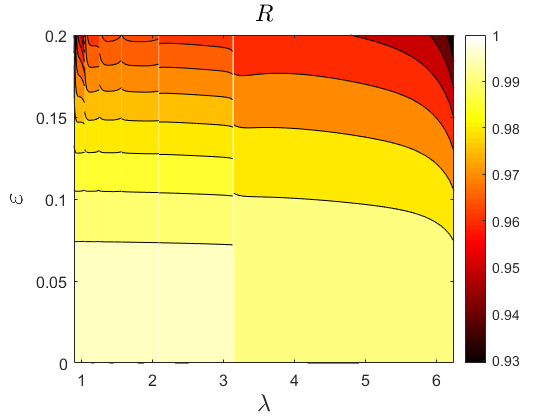
\includegraphics[width=7.6cm]{sections/6_scattering_and_reflectivity/refl_map_N_M_16.png} }}
    \subfloat[\centering Energy Defect]
    {{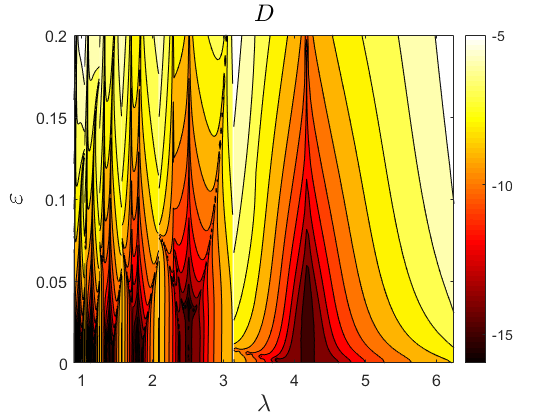
\includegraphics[width=7.6cm]{sections/6_scattering_and_reflectivity/energy_defect_N_M_16.png} }}
    \vspace{3mm}
    \caption{The Reflectivity Map, $R(\varepsilon,\delta)$, and Energy Defect $D$
    computed with Taylor summation. We set $N=M=16$ 
    with a granularity of $N_{\varepsilon}=N_{\delta}=100$ per invocation. The grating surface was $(6.4)$ and physical parameters were $(6.5)$.}
    \label{Fig:RM:Dielectric}
\end{figure}
\vspace{-15mm}
We then changed to non--normal incidence ($\alpha \neq 0$) and increased the granularity to $N_{\varepsilon}=N_{\delta}=1000$ per invocation. In Chapter 7 we will discuss the advantageous computational complexity 
our HOPS/AWE algorithm enjoys in this situation of large $N_{\varepsilon}$ and $N_{\delta}$. We selected
\be
f(x) = \cos(x),
\quad
\varepsilon_{\text{max}}=0.2,
\ee
with the parameters
%\vspace{-32mm}
\be
\alpha = 10^{-4},
\quad
\sigma=0.99,
\quad
n^u=1,
\quad
n^w = 1.1,
\quad N_x = N_z = 32,
\quad N=M=16.
\ee
In Figure $18(\text{a})$ we plot six different subsets of the
Reflectivity Map on a single coordinate axis, and in 
Figure $18(\text{b})$ we plot the Energy Defect
to demonstrate the accuracy of our scheme with
a nonzero value of $\alpha$.
%
% Figure: Reflectivity Map for Vacuum over Dielectric (Fine)
%
\vspace{-17mm}
\begin{figure}[H]
    \centering
    \subfloat[\centering Reflectivity Map]
    {{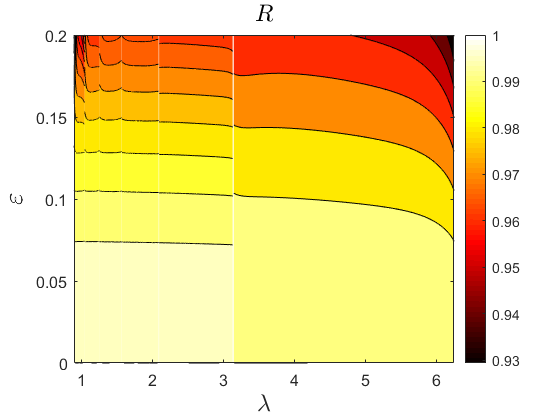
\includegraphics[width=7.6cm]{sections/6_scattering_and_reflectivity/refl_map_N_M_16_nonzero_alpha.png} }}
    \subfloat[\centering Energy Defect ]
    {{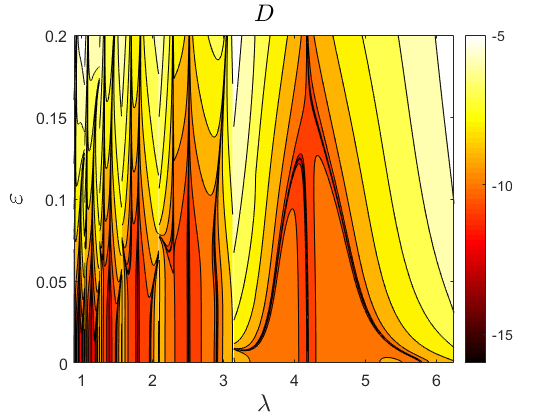
\includegraphics[width=7.6cm]{sections/6_scattering_and_reflectivity/energy_defect_N_M_16_nonzero_alpha.png} }}
    \vspace{3mm}
    \caption{The Reflectivity Map, $R(\varepsilon,\delta)$, and Energy Defect $D$
    computed with Taylor summation. We set $N=M=16$
    with a granularity of $N_{\varepsilon}=N_{\delta}=1000$ per invocation. The grating surface was $(6.6)$ and physical parameters were $(6.7)$.}
    \label{Fig:RM:Dielectric:Fine}
\end{figure}
\vspace{-17mm}
Next, we considered normal incidence ($\alpha = 0$) and changed the lower index of refraction $n^w$ to match representative values
of silver (Ag) and gold (Au) as reported by Johnson \& Christy 
\cite{JohnsonChristy72}, in particular
\bes
n_{\text{Ag}} = 0.05 + 2.275 i,
\quad
n_{\text{Au}} = 1.48 + 1.883i.
\ees
Using the same frequency and wavelength ranges, we studied
\be
f(x) = \cos(4x),
\quad
\varepsilon_{\text{max}} = 0.2,
\ee
with the parameters
\be
\alpha = 0,
\quad
\sigma=0.99,
\quad
n^u = 1,
\quad
N_x = N_z = 32,
\quad
N=M=15.
\ee
In Figure $19(\text{a})$ we plot six different subsets of the Reflectivity
Map where the lower index of refraction is selected to model the optical constant
of silver. In Figure $19(\text{b})$ we plot six different subsets of 
the Reflectivity Map where the lower index of refraction is changed to the optical
constant for gold.
%
% Figure: Reflectivity Map for Metals
%
\vspace{-18mm}
\begin{figure}[H]
    \centering
    \subfloat[\centering Reflectivity Map for Silver]
    {{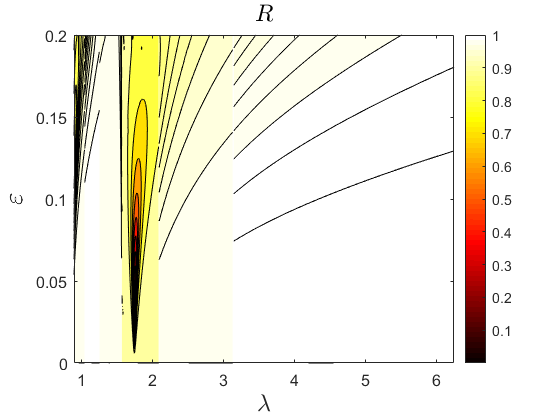
\includegraphics[width=7.6cm]{sections/6_scattering_and_reflectivity/Reflectivity Map for Silver.png} }}
    \subfloat[\centering Reflectivity Map for Gold]
    {{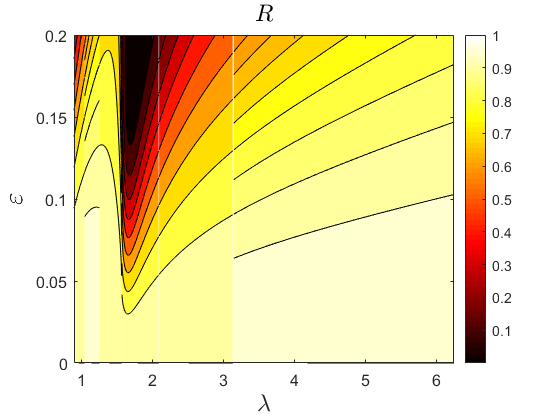
\includegraphics[width=7.6cm]{sections/6_scattering_and_reflectivity/Reflectivity Map for Gold.png} }}
    \vspace{3mm}
    \caption{The Reflectivity Map, $R(\varepsilon,\delta)$, for silver (left)
    and gold (right) with
    Pad\'e summation. We set $N=M=15$ with a granularity
    of $N_{\varepsilon}=N_{\delta}=100$ per invocation. The grating surface was $(6.8)$ and physical parameters were $(6.9)$ with $n^w = n_{\text{Ag}}$ (left)
    and $n^w = n_{\text{Au}}$ (right).}
    \label{Fig:RM:Metal}
\end{figure}
\vspace{-18mm}
We then changed the lower index of refraction $n^w$ to match representative values
of tungsten $(W)$ and iron (Fe) as reported by Ordal et al. \cite{Ordal:88}, where
\bes
n_{\text{W}} = 3.8313 + 2.9043 i,
\quad
n_{\text{Fe}} = 4.274 + 9.579 i.
\ees
From these, we studied
\be
f(x) = \sin(4x),
\quad
\varepsilon_{\text{max}} = 0.2,
\ee
with the parameters
\be
\alpha = 0,
\quad
\sigma=0.99,
\quad
n^u = 1,
\quad
N_x = N_z = 32,
\quad
N=M=15.
\ee
In Figure $20(\text{a})$ we plot six different subsets of the Reflectivity
Map where the lower index of refraction is selected to model the optical constant
of tungsten. In Figure $20(\text{b})$ we plot six different subsets of 
the Reflectivity Map where the lower index of refraction is changed to the optical
constant for iron.
%
% Figure: Reflectivity Map for Metals 2
%
\vspace{-18mm}
\begin{figure}[H]
    \centering
    \subfloat[\centering Reflectivity Map for Tungsten]
    {{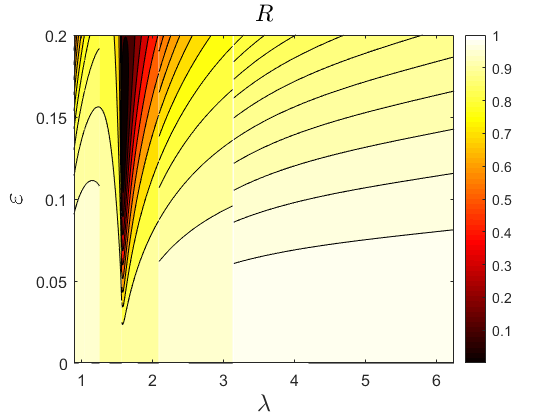
\includegraphics[width=7.6cm]{sections/6_scattering_and_reflectivity/Reflectivity Map for Tungsten.png} }}
    \subfloat[\centering Reflectivity Map for Iron]
    {{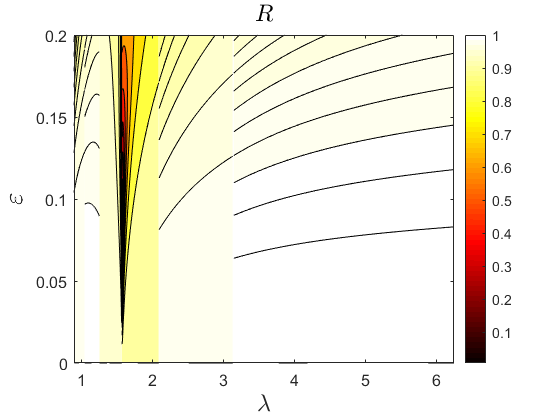
\includegraphics[width=7.6cm]{sections/6_scattering_and_reflectivity/Reflectivity Map for Iron.png} }}
    \vspace{3mm}
    \caption{The Reflectivity Map, $R(\varepsilon,\delta)$, for tungsten (left)
    and iron (right) with
    Pad\'e summation. We set $N=M=15$ with a granularity
    of $N_{\varepsilon}=N_{\delta}=100$ per invocation. The grating surface was $(6.10)$ and physical parameters were $(6.11)$ with $n^w = n_{W}$ (left)
    and $n^w = n_{\text{Fe}}$ (right).}
    \label{Fig:RM:Metal 2}
\end{figure}
\vspace{-18mm}
We then changed back to  non--normal incidence ($\alpha \neq 0$) and reduced our total computation time by simulating $R$ in the following frequency/wavelength ranges
\begin{align*}
q&=1:\quad \omega\in[1.005,1.995] \quad\implies\quad \lambda\in[3.14947,6.25193],\\
q&=2:\quad \omega\in[2.005,2.995] \quad\implies\quad\lambda\in[2.09789,3.13376],\\
q&=3:\quad \omega\in[3.005,3.995] \quad\implies\quad \lambda\in[1.57276,2.09091].
\end{align*}
We selected
\be
f(x) = \cos(3x),
\quad
\varepsilon_{\text{max}}=0.2,
\ee
with the parameters
\be
\alpha = 0.01,
~~
\sigma=0.99,
~~
n^u=1,
~~ 
n^w = 3.1874,
~~
N_x = N_z = 64,
~~
N=M=13,
\ee
and the value of $n^w$ is meant to model Zinc germanium phosphide \cite{das2003linear}.
In Figure $21\text{(a)}$ we plot three different subsets of the Reflectivity
Map on one set of coordinate axes. In Figure $21\text{(b)}$ we plot the
Energy Defect to show the accuracy of our scheme in the case $\alpha \neq 0$.
\vspace{-18mm}
%
% Figure: Reflectivity Map for Vacuum over Silicon
%
\begin{figure}[H]
    \centering
    \subfloat[\centering Reflectivity Map]
    {{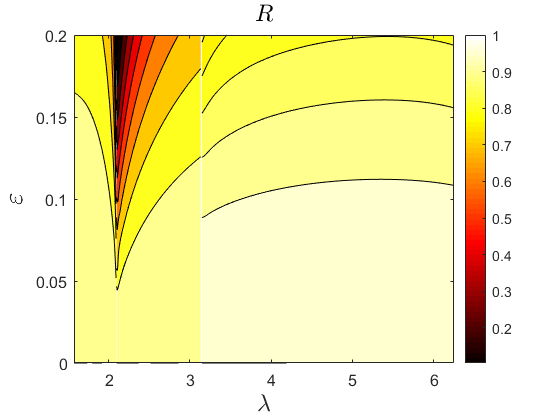
\includegraphics[width=7.6cm]{sections/6_scattering_and_reflectivity/Reflectivity Map Zinc Germanium Phosphide.png} }}
    \subfloat[\centering Energy Defect]
    {{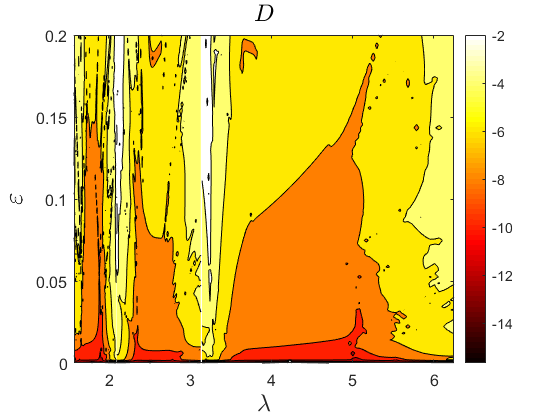
\includegraphics[width=7.6cm]{sections/6_scattering_and_reflectivity/Energy Defect Zinc Germanium Phosphide.png} }}
    \caption{The Reflectivity Map, $R(\varepsilon,\delta)$, and Energy Defect
    $D$ computed with Pad\'e summation. We set 
    $N=M=13$ with a granularity of $N_{\varepsilon}=N_{\delta}=100$ per 
    invocation. The grating surface was $(6.12)$ and physical parameters were $(6.13)$ with $n^w=3.1874$ (Zinc germanium phosphide).}
    \label{Fig:RM:Flint}
\end{figure}

\vspace{-19mm}
\hspace{-6.8mm} Next, we studied
\be
f(x) = \sin(3x),
\quad
\varepsilon_{\text{max}}=0.2,
\ee
with the parameters
\vspace{-0.4mm}
\be
\alpha = 0.01,
~~
\sigma=0.99,
~~
n^u=1,
~~
n^w = 2.1054,
~~
N_x = N_z = 64,
~~
N=M=13,
\ee
\vspace{-0.4mm}
\hspace{-2mm}and the value of $n^w$ is meant to model Zinc monoxide \cite{bond1965measurement}.
In Figure $22\text{(a)}$ we plot three different subsets of the Reflectivity
Map on one set of coordinate axes. In Figure $22\text{(b)}$ we plot the 
Energy Defect to show the accuracy of our scheme in the case $\alpha \neq 0$.
%
% Figure: Reflectivity Map for Vacuum over Flint
%
\vspace{-22.3mm}
\begin{figure}[H]
    \centering
    \subfloat[\centering Reflectivity Map]
    {{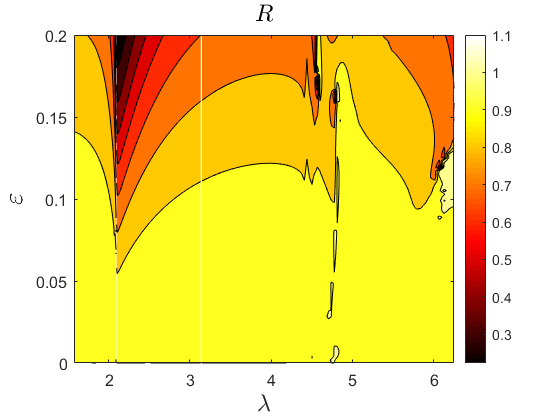
\includegraphics[width=7.6cm]{sections/6_scattering_and_reflectivity/Reflectivity Map Zinc.png} }}
    \subfloat[\centering Energy Defect]
    {{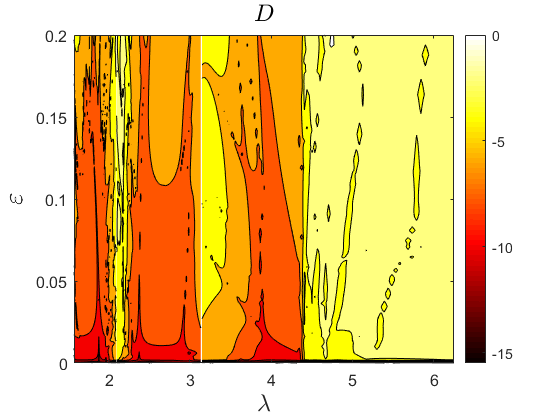
\includegraphics[width=7.6cm]{sections/6_scattering_and_reflectivity/Energy Defect Zinc.png} }}
    %\vspace{3mm}
    \caption{The Reflectivity Map, $R(\varepsilon,\delta)$, and Energy Defect
    $D$ computed with Pad\'e summation. We set 
    $N=M=13$ with a granularity of $N_{\varepsilon}=N_{\delta}=100$ per 
    invocation. The grating surface was $(6.14)$ and physical parameters were $(6.15)$ with $n^w=2.1054$ (Zinc monoxide).}
    \label{Fig:RM:Flint}
\end{figure}
%\newline
%\\
Seeking to understand what occurs for non--physical values of the dielectric constants, we simulated $R$ with the first frequency/wavelength range in $(6.3)$ and selected
\be
f(x) = \cos(x),
\quad
\varepsilon_{\text{max}} = 0.4,
\ee
with the high refractive indices
\be
\alpha = 0,
\quad
\sigma=0.99,
\quad
n^u = 5,
\quad
n^w = 8.1,
\quad
N_x = N_z = 32,
\quad
N=M=12,
\ee
In Figure $23(\text{a})$ we plot a single subset of the
Reflectivity Map on a single coordinate axis, and in 
Figure $23(\text{b})$ we plot the Energy Defect. Our choice of dielectric constants produces an interesting pattern in the computation of $R$.

%
% Figure: Reflectivity Map for Non-Physical Dielectric
%
\vspace{-19mm}
\begin{figure}[H]
    \centering
    \subfloat[\centering Reflectivity Map]
    {{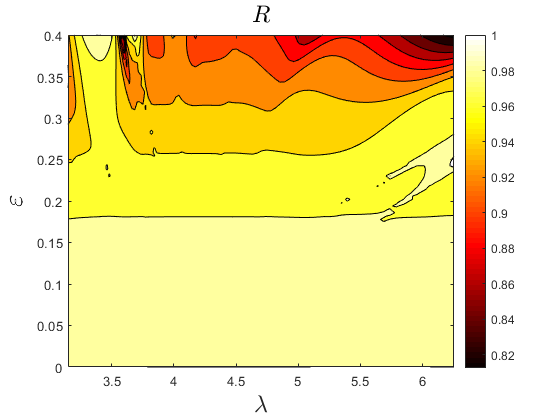
\includegraphics[width=7.6cm]{sections/6_scattering_and_reflectivity/Reflectivity Map Flame.png} }}
    \subfloat[\centering Energy Defect]
    {{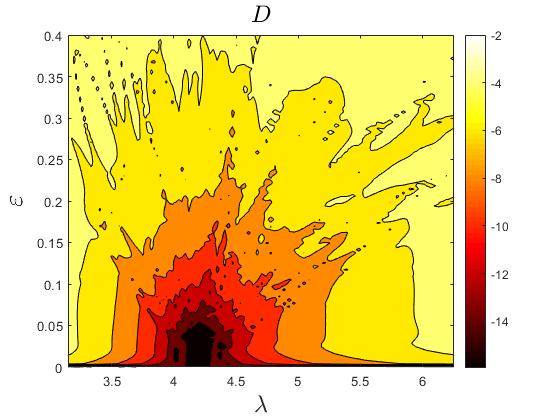
\includegraphics[width=7.6cm]{sections/6_scattering_and_reflectivity/Energy Defect Flame.png} }}
    \vspace{3mm}
    \caption{The Reflectivity Map, $R(\varepsilon,\delta)$, and Energy Defect $D$
    computed with Pad\'e summation. We set $N=M=12$ 
    with a granularity of $N_{\varepsilon}=N_{\delta}=100$ per invocation. The grating surface was $(6.16)$ and physical parameters were $(6.17)$.}
    \label{Fig:RM:Single Case 1}
\end{figure}
\vspace{-18mm}
\hspace{-6mm}We then studied
\be
f(x) = \cos(x),
\quad
\varepsilon_{\text{max}} = 0.2,
\ee
with a purely imaginary index of refraction in the lower layer
\be
\alpha = 0.1,
\quad
\sigma=0.99,
\quad
n^u = 15,
\quad
n^w = 20i,
\quad
N_x = N_z = 32,
\quad
N=M=15.
\ee
In Figure $24(\text{a})$ we plot a single subset of the
Reflectivity Map on a single coordinate axis, and in 
Figure $24(\text{b})$ we plot the Energy Defect, where we once again observe an interesting pattern generated through our choice of dielectric constants. As the lower refractive index, $n^w$, is purely imaginary, we do not expect that $(6.2)$ holds and $D\neq 0$. Nonetheless, we still found scattered energy in the far--field and small values of $D$ when the value of $n^w$ is purely imaginary.


%
% Figure: Reflectivity Map for Non-Physical Dielectric
%
\vspace{-16mm}
\begin{figure}[H]
    \centering
    \subfloat[\centering Reflectivity Map]
    {{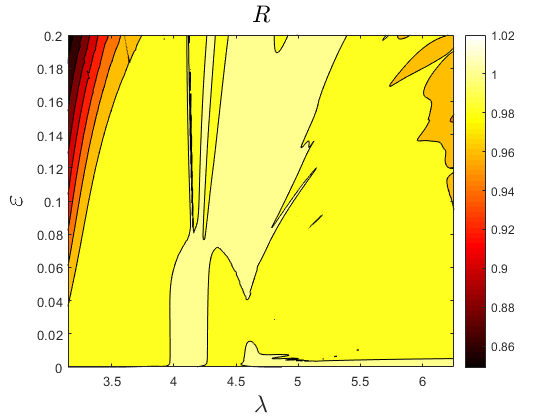
\includegraphics[width=7.6cm]{sections/6_scattering_and_reflectivity/Reflectivity Map TM Single Case 1.png} }}
    \subfloat[\centering Energy Defect]
    {{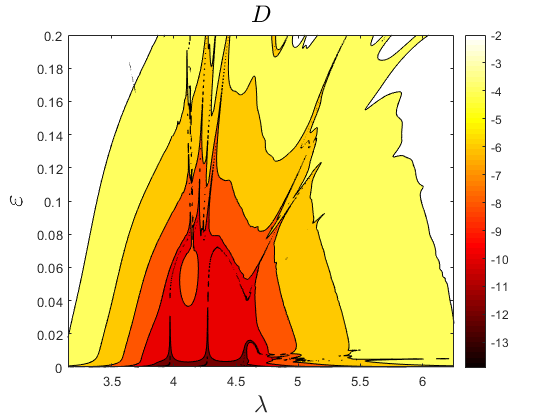
\includegraphics[width=7.6cm]{sections/6_scattering_and_reflectivity/Energy Defect TM Single Case 1.png} }}
    \vspace{2mm}
    \caption{The Reflectivity Map, $R(\varepsilon,\delta)$, and Energy Defect $D$
    computed with Pad\'e summation. We set $N=M=15$ 
    with a granularity of $N_{\varepsilon}=N_{\delta}=1000$ per invocation. The grating surface was $(6.18)$ and physical parameters were $(6.19)$.}
    \label{Fig:RM:Single Case 1}
\end{figure}
\vspace{-18mm}
\hspace{-6mm}Finally, we selected
\be
f(x) = \sin(x),
\quad
\varepsilon_{\text{max}} = 0.2,
\ee
with the parameters
\be
\alpha = 0.1,
\quad
\sigma=0.99,
\quad
n^u = 10,
\quad
n^w = 40i,
\quad
N_x = N_z = 32,
\quad
N=M=20.
\ee
In Figure $25(\text{a})$ we plot a single subset of the
Reflectivity Map and in 
Figure $25(\text{b})$ we plot the Energy Defect.


%
% Figure: Reflectivity Map for Non-Physical Dielectric
%
\vspace{-22mm}
\begin{figure}[H]
    \centering
    \subfloat[\centering Reflectivity Map]
    {{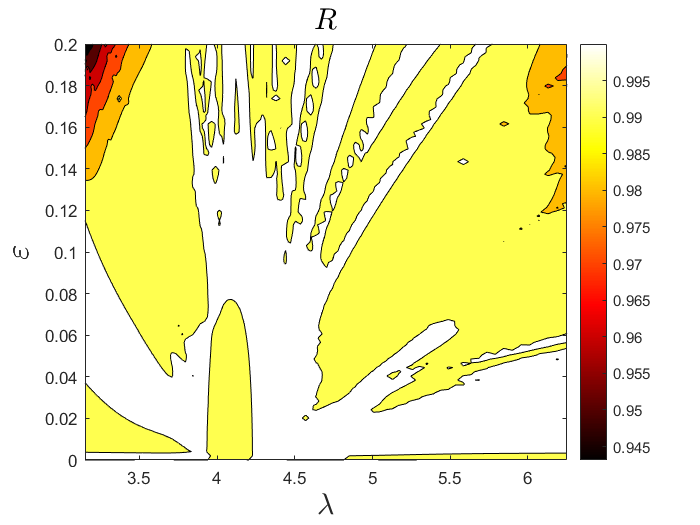
\includegraphics[width=7.6cm]{sections/6_scattering_and_reflectivity/Reflectivity Map TM Single Case 2.png} }}
    \subfloat[\centering Energy Defect]
    {{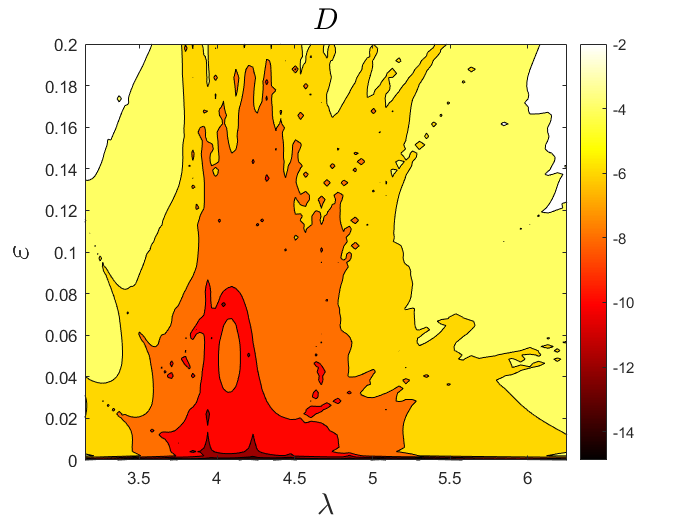
\includegraphics[width=7.6cm]{sections/6_scattering_and_reflectivity/Energy Defect TM Single Case 2.png} }}
    \vspace{2mm}
    \caption{The Reflectivity Map, $R(\varepsilon,\delta)$, and Energy Defect $D$
    computed with Pad\'e summation. We set $N=M=20$ 
    with a granularity of $N_{\varepsilon}=N_{\delta}=100$ per invocation. The grating surface was $(6.20)$ and physical parameters were $(6.21)$.}
    \label{Fig:RM:Single Case 2}
\end{figure}